\documentclass[11pt, a4paper]{article}

% Packages
\usepackage[francais]{babel}
\usepackage[T1]{fontenc}
\usepackage[utf8]{inputenc}

\usepackage[left=2cm, right=2cm, top=2cm, bottom=2cm]{geometry}
\usepackage{fancyhdr}
\usepackage{lastpage}
\usepackage{hyperref}
\usepackage{float}
\usepackage{graphicx}
\graphicspath{{./img/}}
\usepackage{multicol}

% Reset paragraph indentation -------------------------------------------------
\setlength{\parindent}{0cm}

% Page header and footer ------------------------------------------------------
\pagestyle{fancy}
\setlength{\headheight}{14pt}
\renewcommand{\headrulewidth}{0.5pt}
\lhead{Programmation temps-réel}
%\lhead{\includegraphics[height=1cm]{logo.jpg}} % Change \headheight to right size
\chead{Émetteur et récepteur lumineux}
\rhead{Claudio Sousa, David Gonzalez}
\renewcommand{\footrulewidth}{0.5pt}
\lfoot{17/05/2018}
\cfoot{Groupe 3}
\rfoot{Page \thepage /\pageref{LastPage}}

% Table of contents depth -----------------------------------------------------
\setcounter{tocdepth}{3}

% Document --------------------------------------------------------------------
\begin{document}

\title
{
    \Huge{Programmation temps-réel} \\
    \Huge{Émetteur et récepteur lumineux}
}
\author
{
    \LARGE{Claudio Sousa, David Gonzalez - Groupe 3}
}
\date{17/05/2018}
\maketitle

\thispagestyle{empty}

\section{État du projet}

Le projet est en état de marche et
toutes les fonctionnalités ont pu être implémentées. \\

L'émetteur fonctionne sans soucis.

Les 4 tâches du récepteur fonctionnent également bien, y compris sous forte charge.

\section{Anomalies ou bugs}

Les programmes fonctionnent sans anomalie.

\section{Traces sous forte charge}

\subsection{Déroulement}

Une trace complète a été prise à chaque étape de charge de l'émetteur afin de pouvoir comparer les effets.
Voici donc ci-dessous 4 fois la trace avec les 4 sections (étapes) mise en évidence:

\begin{figure}[H]
    \begin{center}
        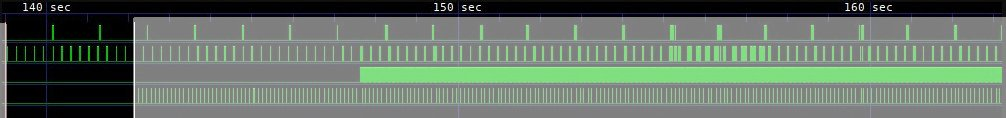
\includegraphics[width=1\textwidth]{global_section1_empty}
        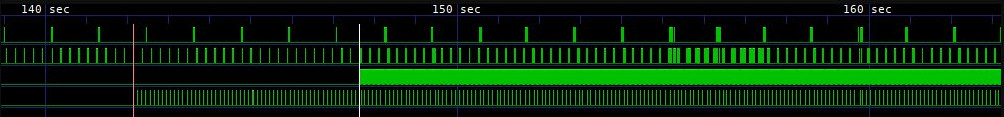
\includegraphics[width=1\textwidth]{global_section2_leds}
        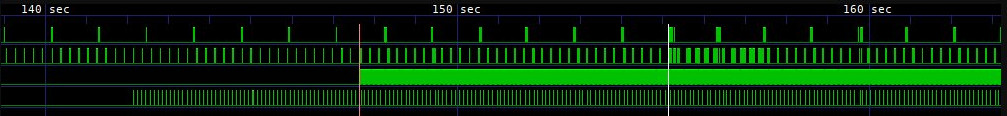
\includegraphics[width=1\textwidth]{global_section3_load}
        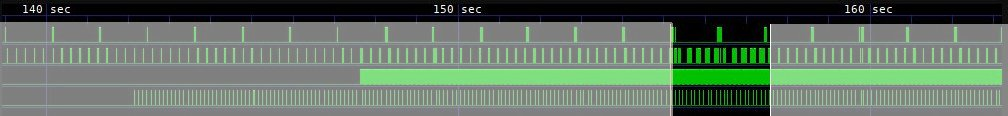
\includegraphics[width=1\textwidth]{global_section4_send}
    \end{center}
    \caption{Déroulement et traces globales sectionnées en 4 parties}
    \label{Déroulement et traces globales sectionnées en 4 parties}
\end{figure}

Ces sections décrivent le déroulement de l'opération.
Tout d'abord, le récepteur a été mis en marche avec les paramètres suivants:
\begin{itemize}
    \item scroll fast (220 ms);
    \item load 0;
    \item leds off. \\
\end{itemize}

La première section est celle avec les paramètres décrits ci-dessus. \\
La deuxième section est lorsque la tâche des LEDs a été mise en marche (\textit{leds on}). \\
La troisième section est lorsque la tâche de charge (load) a été mise en marche (\textit{load 15}). \\
La quatrième et dernière section est celle où une commande \textit{send} a été envoyée (\textit{send test.txt}). \\

\subsection{Section 1}

Voici un zoom sur la section 1 avec les timings de chacune des tâches en exécution:

\begin{figure}[H]
    \begin{multicols}{2}
        \begin{center}
            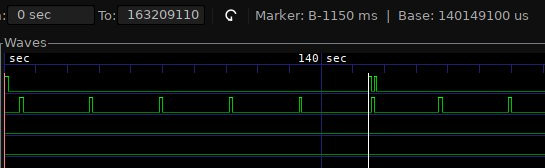
\includegraphics[width=0.5\textwidth]{section1_empty_t1_light}
        \end{center}
        \columnbreak
        \begin{center}
            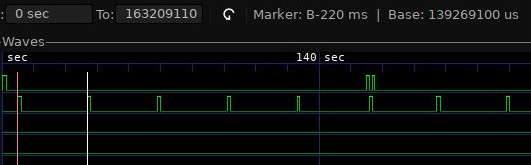
\includegraphics[width=0.5\textwidth]{section1_empty_t2_cmd}
        \end{center}
    \end{multicols}
    \caption{Zoom sur la section 1}
    \label{Zoom sur la section 1}
\end{figure}

Seules deux tâches sont en exécution, puisque à ce stade, la tâche des LEDs et la tâche de charge ne sont pas actives. \\

Ici, le processeur ne fait pas grand chose et a largement le temps d'exécuter toutes les tâches en cours et
de respecter les timings de la tâche 2 (commande à 220 ms).

\subsection{Section 2}

Voici un zoom sur la section 2 avec les timings de chacune des tâches en exécution:

\begin{figure}[H]
    \begin{multicols}{2}
        \begin{center}
            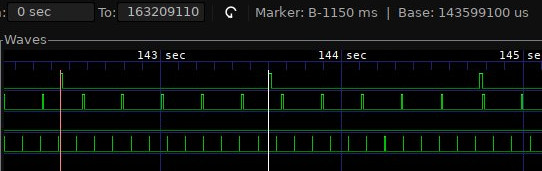
\includegraphics[width=0.5\textwidth]{section2_leds_t1_light}
        \end{center}
        \columnbreak
        \begin{center}
            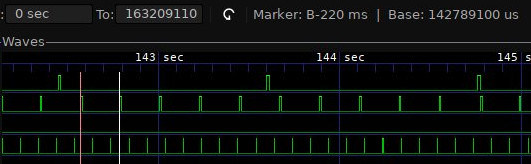
\includegraphics[width=0.5\textwidth]{section2_leds_t2_cmd}
        \end{center}
    \end{multicols}
    \begin{center}
        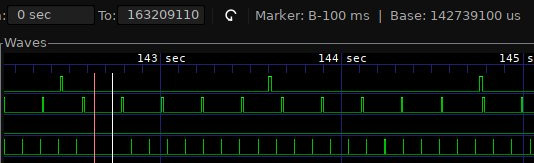
\includegraphics[width=0.5\textwidth]{section2_leds_t4_leds}
    \end{center}
    \caption{Zoom sur la section 2}
    \label{Zoom sur la section 2}
\end{figure}

Pas grand chose a dire de plus par rapport à la première section.
En effet, la tâche 4 (LEDs) a été activée, mais son temps d'exécution étant négligeable,
elle n'affecte en rien le système.

\subsection{Section 3}

Voici un zoom sur la section 3 avec les timings de chacune des tâches en exécution:

\begin{figure}[H]
    \begin{multicols}{2}
        \begin{center}
            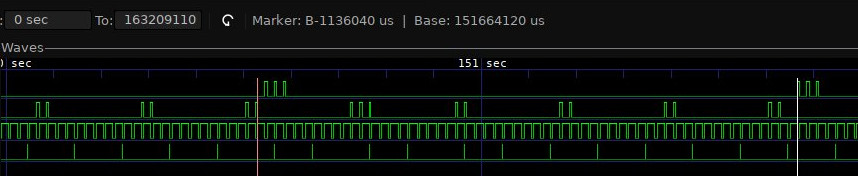
\includegraphics[width=0.5\textwidth]{section3_load_t1_light}
        \end{center}
        \columnbreak
        \begin{center}
            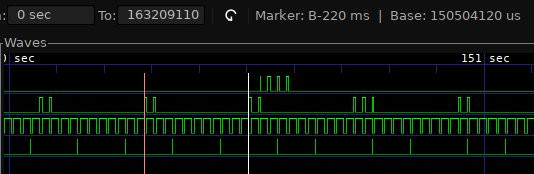
\includegraphics[width=0.5\textwidth]{section3_load_t2_cmd}
        \end{center}
    \end{multicols}
    \begin{multicols}{2}
        \begin{center}
            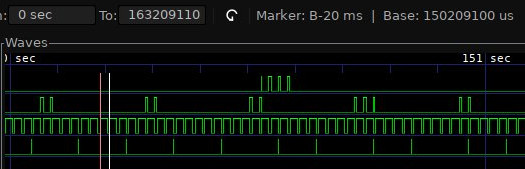
\includegraphics[width=0.5\textwidth]{section3_load_t3_load}
        \end{center}
        \columnbreak
        \begin{center}
            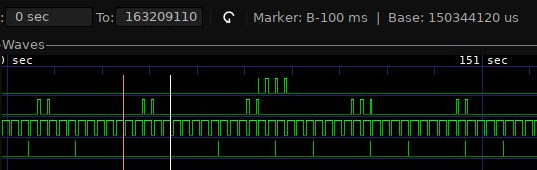
\includegraphics[width=0.5\textwidth]{section3_load_t4_leds}
        \end{center}
    \end{multicols}
    \caption{Zoom sur la section 3}
    \label{Zoom sur la section 3}
\end{figure}

Ici, la tâche 3 (load) a été activée à son maximum (15 ms).
On remarque tout de suite que les tâches ne peuvent plus être exécuté d'un trait à cause de la tâche de charge et
ralonge par conséquent le temps de réponse, mais en respectant les timings.

\subsection{Section 4}

La section 4 est le plus chargée de toutes avec la commande \textit{send} envoyée. \\

Selon le trace ci-dessous, la tâche 1 a largement le temps de s'exécuter.
On remarque un peu de gigue temporel, mais la cadence étant donnée par le DMA du décodeur,
la charge du CPU ne fait que retarder le décodage du message et n'affecte en rien la réception.

\begin{figure}[H]
    \begin{multicols}{2}
        \begin{center}
            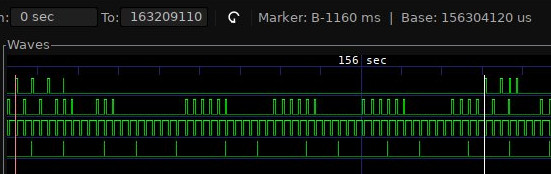
\includegraphics[width=0.5\textwidth]{section4_send_t1_light_1}
        \end{center}
        \columnbreak
        \begin{center}
            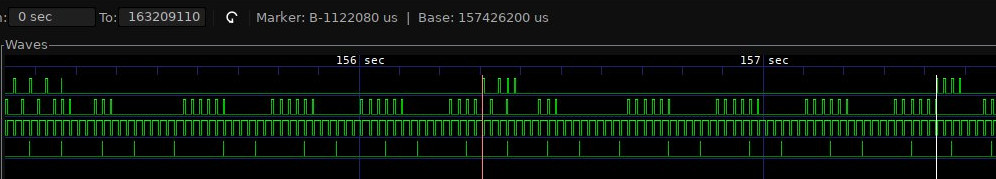
\includegraphics[width=0.5\textwidth]{section4_send_t1_light_2}
        \end{center}
    \end{multicols}
    \caption{Zoom sur la section 4, tâche 1}
    \label{Zoom sur la section 4, tâche 1}
\end{figure}

Concernant la tâche 2, la trace nous montre que son temps de réponse est d'environ 110 ms.
Aucune gigue n'a pas été observée, mais même en cas de décalage, le tâche à de la marge.

\begin{figure}[H]
    \begin{multicols}{2}
        \begin{center}
            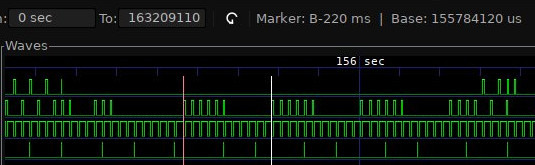
\includegraphics[width=0.5\textwidth]{section4_send_t2_cmd_1}
        \end{center}
        \columnbreak
        \begin{center}
            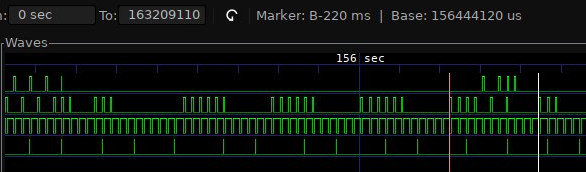
\includegraphics[width=0.5\textwidth]{section4_send_t2_cmd_2}
        \end{center}
    \end{multicols}
    \caption{Zoom sur la section 4, tâche 2}
    \label{Zoom sur la section 4, tâche 2}
\end{figure}

Concernant la tâche 3, son timings est parfait, puisque c'est la tâche avec la plus haute priorité.

\begin{figure}[H]
    \begin{multicols}{2}
        \begin{center}
            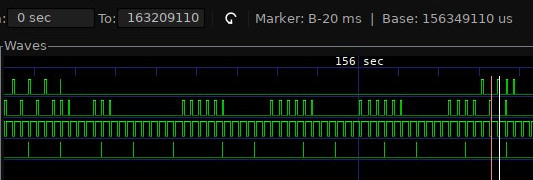
\includegraphics[width=0.5\textwidth]{section4_send_t3_load_1}
        \end{center}
        \columnbreak
        \begin{center}
            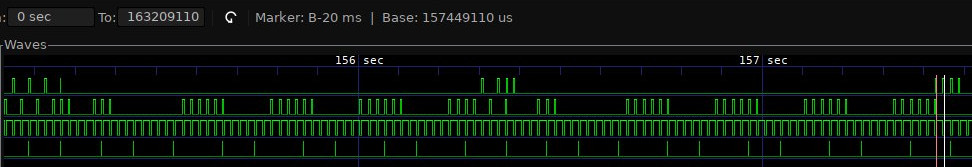
\includegraphics[width=0.5\textwidth]{section4_send_t3_load_2}
        \end{center}
    \end{multicols}
    \caption{Zoom sur la section 4, tâche 3}
    \label{Zoom sur la section 4, tâche 3}
\end{figure}

Finalement, pour la tâche 4, on observe sur la trace une gigue d'environ 20 ms.
En effet, la tâche n'arrive pas a garder son timings parfait de 100 ms à cause de la charge.
Cependant, ce n'est qu'un gigue, soit positive ou négative, comme observé sur la trace ci-dessous:

\begin{figure}[H]
    \begin{multicols}{2}
        \begin{center}
            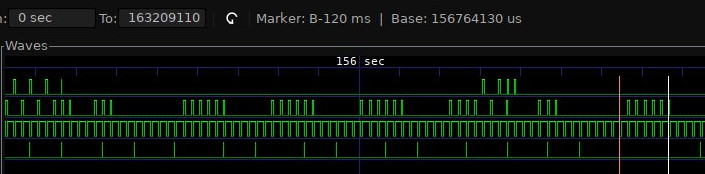
\includegraphics[width=0.5\textwidth]{section4_send_t4_leds_2}
        \end{center}
        \columnbreak
        \begin{center}
            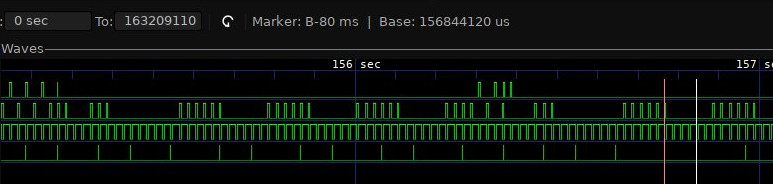
\includegraphics[width=0.5\textwidth]{section4_send_t4_leds_3}
        \end{center}
    \end{multicols}
    \caption{Zoom sur la section 4, tâche 4}
    \label{Zoom sur la section 4, tâche 4}
\end{figure}

Par ailleurs, lorsque la forte charge est passée, la tâche récupère bien son timings:

\begin{figure}[H]
    \begin{center}
        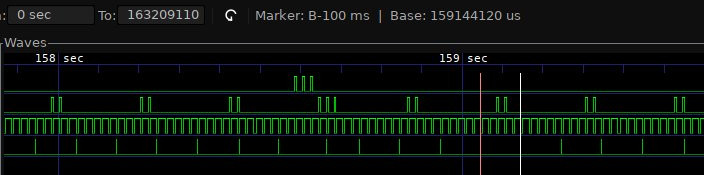
\includegraphics[width=0.7\textwidth]{section4_send_t4_leds_5}
    \end{center}
    \caption{Récupération du timings de la tâche 4}
    \label{Récupération du timings de la tâche 4}
\end{figure}

\end{document}
